\section{Results}
% Figures are exported to figures/ as PDF (for example by an analysis
% script) and included by name; \graphicspath points there.
\begin{figure*}[htbp]
\centering
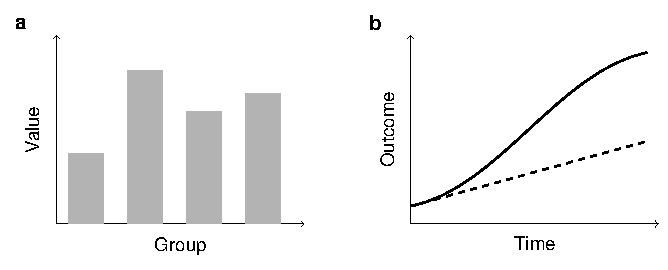
\includegraphics[width=0.7\textwidth]{example.pdf}
\caption{Study overview. \textbf{a}, What the first panel shows.
\textbf{b}, What the second panel shows.}
\label{fig:overview}
\end{figure*}

\paragraph{Main finding.} Describe the main result with its estimate and
interval (\cref{fig:overview}a, \cref{tab:results}). Details are in
Supplementary \cref{S-tab:supp-details} and Supplementary
\cref{S-fig:supp-flow}, and the additional analysis in Supplementary
\cref{S-note:supp-method}.

% Tables live in tables/, one file per table, so scripts can regenerate them.
\begin{table}[htbp]
\centering
\footnotesize
\caption{Main results. Estimates with 95\% confidence intervals (CI).
\textbf{Bold}: \textit{p}\textsubscript{adj}\,<\,0.05.}
\label{tab:results}
% Shrinks the table to the column width only when it is wider.
\resizebox{\ifdim\width>\columnwidth \columnwidth\else\width\fi}{!}{%
\begin{tabular}{lcc}
\toprule
\textbf{Method} & \textbf{Estimate (95\% CI)} & \textbf{Adjusted p} \\
\midrule
Proposed & \textbf{0.62 (0.60--0.63)} & <0.001 \\
Baseline & 0.33 (0.32--0.34) & -- \\
\bottomrule
\end{tabular}}
\end{table}


\paragraph{Secondary finding.} Describe it the same way (\cref{fig:overview}b).
